\documentclass[conference]{IEEEtran}
\usepackage{cite}
\usepackage{amsmath,amssymb,amsfonts}
\usepackage{array}
\usepackage{graphicx}
\usepackage{booktabs}
\usepackage{multirow}
\usepackage{xcolor}
\usepackage{url}
\usepackage{balance}
\usepackage{enumitem}
\usepackage{tikz}
\usetikzlibrary{arrows.meta,positioning,shapes.geometric}

\newcommand{\gate}{\mathcal{G}}
\newcommand{\ind}{\mathbb{1}}
\newcommand{\score}{\mathcal{P}}

\begin{document}

\title{Is De-Extinction Possible? ProxyGate: An Evidence-Gated Research Design for Extinct-Species Proxies}

\author{\IEEEauthorblockN{Research Proposal Generated from a Four-Agent Evidence-to-Design Workflow}
\IEEEauthorblockA{Survey $\rightarrow$ Idea $\rightarrow$ ExperimentDesign $\rightarrow$ Author\\
Paleogenomics, conservation decision science, and governance research plan}}

\maketitle

\begin{abstract}
De-extinction is commonly presented as a yes-or-no technical question, although the label covers biologically different acts: cloning, selective back-breeding, genome editing of an extant relative, and ecological replacement. This paper proposes ProxyGate, an evidence-gated research design for assessing extinct-species proxies without claiming that a historical organism can be recovered. The central claim is testable: a candidate can be conditionally reviewable only if conservative evidence bounds clear five non-compensatory gates--genomic provenance, trait-to-function support, developmental and welfare protection, ecological counterfactual benefit, and governance with opportunity-cost accountability. A robust priority index is calculated only after all gates pass. The design compares recent-extinction, mammoth-like, deeper-time, and non-avian-dinosaur negative-control classes, and contrasts proxy claims with conventional conservation alternatives. The proposed study is computational and evidence-synthesis only; it reports no edited genomes, embryos, animals, releases, or observed ecological outcomes. The expected contribution is not a promise to resurrect species. It is an auditable way to separate scientifically impossible, evidence-insufficient, and conditionally reviewable proxy hypotheses.
\end{abstract}

\begin{IEEEkeywords}
de-extinction, ancient DNA, conservation genomics, rewilding, decision analysis, animal welfare, governance, uncertainty
\end{IEEEkeywords}

\section{Introduction}

The question ``Is de-extinction possible?'' has unusual public force because it appears to join paleontology, biotechnology, conservation, and science fiction in one sentence. It is nevertheless a poor scientific decision question. ``De-extinction'' may mean recovery of cryopreserved cells from a recently extinct lineage, selective breeding for a historical phenotype, genome editing of an extant relative, or creation of a population intended to supply a lost ecological function. These activities do not share the same evidentiary route, biological object, welfare burden, or legal status. Their conflation encourages a false choice between a spectacular technological success and categorical impossibility.

This proposal takes a more useful position. An edited or selectively bred descendant of an extant lineage may someday be hypothesized to act as an \emph{extinct-species proxy}; it is not thereby a recovered historical individual. The proxy framing is consistent with the IUCN's terminology of creating proxies of extinct species for conservation benefit \cite{iucn2016}. The distinction is not semantic caution. It determines the evidence that must be supplied. A recoverable DNA fragment is not a complete genome; a reconstructed genome is not a developmental system; a phenotype is not a self-sustaining population; and a population is not automatically a conservation benefit.

Ancient-DNA research has produced striking evidence about extinct populations. It has also shown why molecular recovery cannot be treated as biological reversal. Allentoft \emph{et al.} measured DNA decay in dated bone and found an exponential relationship with major preservation variation among specimens \cite{allentoft2012}. Kistler \emph{et al.} further show that tissue and environment shape ancient-DNA survival patterns \cite{kistler2017}. Mammoth paleogenomics has reconstructed major branches of evolutionary history \cite{vanderValk2021}, and population studies document demographic decline, genetic structure, and genomic erosion in woolly mammoths \cite{palkopoulou2015,dehasque2024}. Such achievements expand what can be inferred about an extinct lineage. They do not restore a cell, a maternal environment, learned behavior, social development, microbiome, or an ecological community.

The core problem is therefore a decision problem under heterogeneous uncertainty. A proposal can have excellent sequence data but no defensible phenotype bridge, no acceptable welfare pathway, no locally credible ecological benefit, or no legitimate governance. A simple weighted score would permit a high genomic score to compensate for a welfare or rights failure. That is a category error. ProxyGate instead uses gates for non-compensatory conditions and applies quantitative prioritization only after all gates pass.

This report is the Author-stage output of a four-agent research workflow. The Survey stage assembled a bounded source registry and gap ledger; the Idea stage compared alternatives and selected an evidence-gated framework; the ExperimentDesign stage specified a computational, design-only evaluation. The present paper organizes those artifacts into a research proposal. It does not report an implemented genetic, reproductive, animal, or ecological experiment.

\section{Evidence Boundary and Research Gap}

\subsection{DNA survival constrains claims, not only dates}

Ancient DNA is chemically modified and fragmented. Allentoft \emph{et al.} estimated a mean half-life for a 242-bp mitochondrial sequence in a geographically constrained moa-bone series and stressed taphonomic variance \cite{allentoft2012}. Their estimate is not a universal stopwatch: preservation environment, tissue, molecular type, and post-mortem history matter. Kistler \emph{et al.} used paleogenomic meta-analysis to show that deamination and fragmentation patterns do not reduce to a single simple chronological rule \cite{kistler2017}. Together, these sources support a direct conclusion: evidence quality must be recorded at the molecule and reconstruction level rather than inferred from a public-facing age label.

This conclusion does not deny exceptional ancient-DNA discoveries. Van der Valk \emph{et al.} recovered million-year-scale mammoth genomic information that substantially refined mammoth evolutionary history \cite{vanderValk2021}. Environmental DNA can also reveal ancient ecosystem composition under favorable mineral-binding conditions \cite{kjaer2022}. But an environmental sequence signal, a damaged fragment, a consensus genome, and a viable diploid cell are scientifically different objects. The sequence of implications is not reversible:

\begin{equation}
\begin{aligned}
\text{molecular evidence} &\Rightarrow \text{bounded evolutionary inference}\\
&\not\Rightarrow \text{recovered organism}.
\end{aligned}
\label{eq:dna-boundary}
\end{equation}

Equation~\eqref{eq:dna-boundary} is a logical boundary, not a claim that every ancient-DNA sample is uninformative. It explains why non-avian dinosaurs should serve as a negative-control class in a decision study. Fossils can deliver morphology, phylogeny, and paleoecological information, but the deep temporal separation from living organisms precludes a credible route from fossil DNA to an exact dinosaur genome or developmental system.

\subsection{Genomes do not settle organismal fidelity}

Paleogenomics makes comparative hypotheses possible, but it does not by itself validate a phenotype, behavior, or ecosystem effect. A proxy derived from an extant relative would inherit the extant lineage's cellular and maternal context. Regulatory architecture, epistasis, pleiotropy, developmental timing, mitochondrial interactions, microbiome, parental care, and social learning can all matter for an organism-level trait. Population history adds another layer. Palkopoulou \emph{et al.} found demographic and genetic decline through woolly mammoth genomes \cite{palkopoulou2015}; Dehasque \emph{et al.} report gradual accumulation of mildly deleterious mutations in the isolated Wrangel Island population \cite{dehasque2024}. A single reference sequence is neither a complete historical population nor a validated blueprint for adaptive potential.

The gap is operational: current discussions often move directly from a reconstructed variant to a claimed trait, then from the trait to ecological restoration. ProxyGate breaks this chain into independently auditable evidence cards. Each card must distinguish observed sequence, reconstructed sequence, phenotype support, unresolved dependencies, and conservation/governance context. A proposed trait that rests on imputation or analogy remains a proposed trait, not an observed property.

\subsection{Functional benefit is a counterfactual, not a label}

Conservation interest is strongest when a candidate might restore a lost function, not when it resembles a well-known extinct form. Yet functional resemblance is neither necessary nor sufficient for ecological benefit. Trophic rewilding literature describes pathways through which large animals can alter food webs and ecosystem processes, while also emphasizing sparse, context-specific, and geographically biased empirical evidence \cite{svenning2016}. Steeves \emph{et al.} argue that functional proxies need sufficient genetic diversity and evolutionary potential to persist rather than merely survive a first generation \cite{steeves2017}.

Consequently, a conservation claim must answer a counterfactual question: compared with habitat protection, protection of extant relatives, translocation, assisted gene flow, invasive-species control, or another feasible portfolio, does the proxy plausibly deliver a net benefit in a specified system? The alternative portfolio is not a rhetorical obstacle. It identifies the conservation opportunity cost of a technologically compelling but ecologically weak project.

\subsection{Welfare and legitimacy require gate status}

Governance analysis finds perceived hazards, moral-hazard concerns, and uncertainty about development paths central to expert views of de-extinction \cite{valdez2019}. Legal and ethical work similarly identifies tensions between revived or modified organisms and existing conservation categories \cite{sherkow2013,camacho2014}. For culturally significant species, genomic stewardship and relationships with rights-holders cannot be reduced to a downstream consent form \cite{collierrobinson2019}. These sources motivate a methodological choice: welfare, rights, governance, and opportunity cost are non-compensatory constraints. If they fail, an appealing genomic narrative does not make a proposal ready for further review.

Table~\ref{tab:gaps} summarizes the evidence-derived gap ledger.

\begin{table*}[t]
\caption{Evidence-derived gaps and their design consequences.}
\label{tab:gaps}
\centering
\footnotesize
\setlength{\tabcolsep}{3pt}
\begin{tabular}{p{0.08\textwidth} p{0.36\textwidth} p{0.46\textwidth}}
\toprule
\textbf{ID} & \textbf{Research gap} & \textbf{ProxyGate response} \\
\midrule
G1 & One label conflates cloning, back-breeding, genome editing, and ecological replacement. & Classify the claim before assessing feasibility; prohibit literal-restoration language unsupported by the evidence. \\
G2 & Reconstruction uncertainty is not routinely propagated from DNA evidence to trait claims. & Evidence cards separate observed, reconstructed, and unknown sequence/trait states. \\
G3 & Genomic similarity is not a validated proxy-fidelity metric. & Require a trait-to-function bridge with independent phenotype and ecology evidence. \\
G4 & Developmental, welfare, and multigenerational uncertainty are separated from technical feasibility. & Use a dedicated welfare/development gate with mandatory human review. \\
G5 & Ecological-benefit claims are insufficiently counterfactual and site-specific. & Compare scenario-based benefit against conventional conservation portfolios. \\
G6 & Governance, participation, and opportunity cost are narrative afterthoughts. & Require rights, legitimacy, stewardship, and resource-allocation evidence as a gate. \\
G7 & No standard benchmark distinguishes impossible, premature, and reviewable proposals. & Test decision categories with negative controls, stress tests, and abstention logic. \\
\bottomrule
\end{tabular}
\end{table*}

\section{ProxyGate Hypothesis and Architecture}

\subsection{Research propositions}

The selected primary idea is **ProxyGate: Evidence-Gated Readiness Assessment for De-Extinction Proxies**. It has two research propositions.

\begin{itemize}[leftmargin=*,nosep]
\item \textbf{H1: Non-compensation.} A candidate should be conditionally reviewable only if each required gate clears a conservative threshold under uncertainty. Strong genomic evidence may increase research value, but it cannot compensate for a developmental, welfare, ecological, or governance failure.
\item \textbf{H2: Counterfactual discipline.} Explicit comparison against conventional conservation portfolios will change the decision category for some apparently attractive proxy claims.
\end{itemize}

These propositions can fail. If all candidates passing a genome-centered screen automatically pass ProxyGate, the additional architecture supplies no discriminating value. If an ecological comparator never changes a decision, it is either redundant or improperly specified. Conversely, if a candidate with rich paleogenomic evidence is routed to `REQUIRES EVIDENCE` because its trait-function bridge or welfare basis is weak, that is a meaningful and intended output--not a negative result to be hidden.

\subsection{Five non-compensatory gates}

Fig.~\ref{fig:proxygate} presents the architecture. A candidate claim first passes through five evidence domains. The final decision is an evidence status, not a permit. `CONDITIONALLY REVIEWABLE` only means that further multidisciplinary human review is scientifically warranted; it does not authorize animal creation, animal use, or environmental release.

\begin{figure*}[t]
\centering
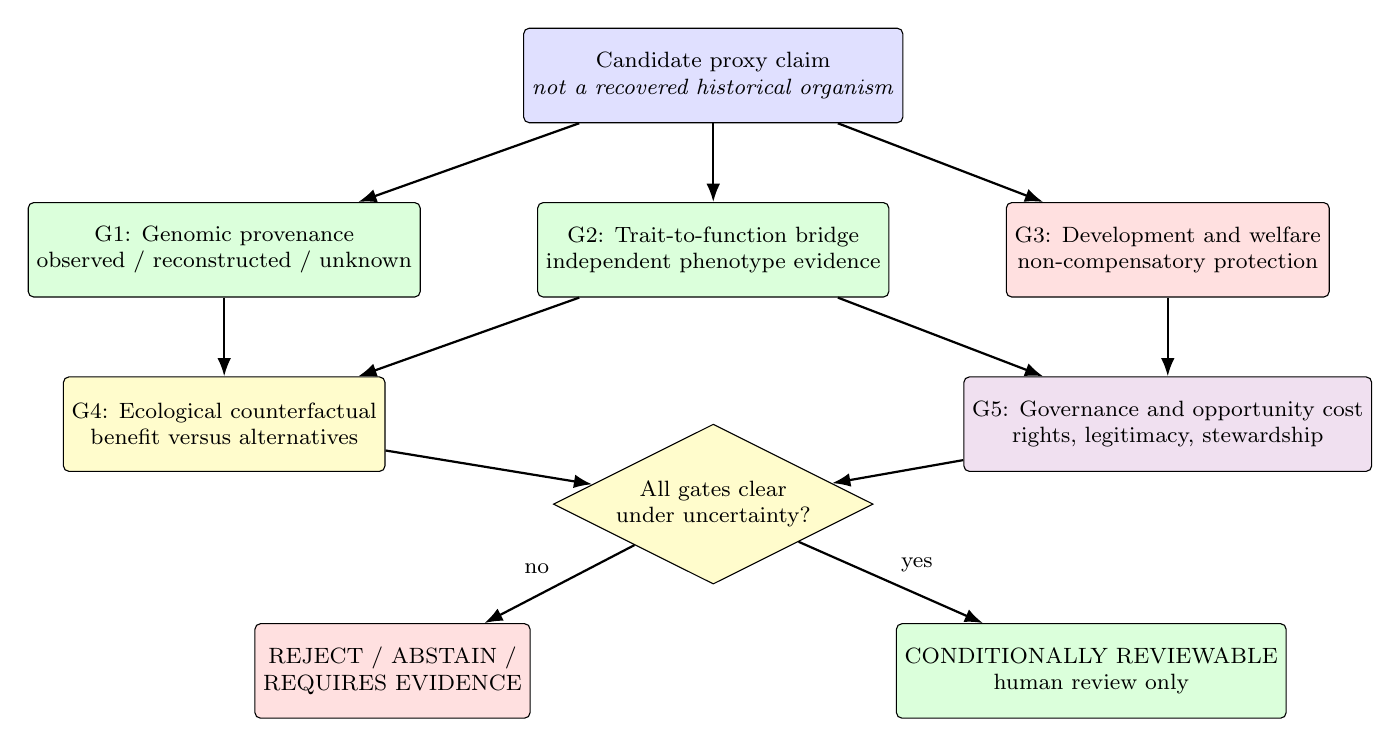
\begin{tikzpicture}[font=\footnotesize, node distance=10mm and 13mm, >=Latex,
  box/.style={draw, rounded corners=2pt, align=center, minimum width=34mm, minimum height=12mm, inner sep=3pt},
  decision/.style={draw, diamond, aspect=2.0, align=center, inner sep=2pt, minimum width=32mm, minimum height=12mm},
  line/.style={->, thick}]
\node[box, fill=blue!12] (claim) {Candidate proxy claim\\\emph{not a recovered historical organism}};
\node[box, fill=green!14, below left=of claim] (genome) {G1: Genomic provenance\\observed / reconstructed / unknown};
\node[box, fill=green!14, below=of claim] (trait) {G2: Trait-to-function bridge\\independent phenotype evidence};
\node[box, fill=red!12, below right=of claim] (welfare) {G3: Development and welfare\\non-compensatory protection};
\node[box, fill=yellow!20, below=of genome] (ecology) {G4: Ecological counterfactual\\benefit versus alternatives};
\node[box, fill=violet!12, below=of welfare] (governance) {G5: Governance and opportunity cost\\rights, legitimacy, stewardship};
\node[decision, fill=yellow!20, below=16mm of trait] (all) {All gates clear\\under uncertainty?};
\node[box, fill=red!12, below left=of all] (no) {REJECT / ABSTAIN /\\REQUIRES EVIDENCE};
\node[box, fill=green!14, below right=of all] (yes) {CONDITIONALLY REVIEWABLE\\human review only};
\draw[line] (claim) -- (genome);
\draw[line] (claim) -- (trait);
\draw[line] (claim) -- (welfare);
\draw[line] (genome) -- (ecology);
\draw[line] (trait) -- (ecology);
\draw[line] (trait) -- (governance);
\draw[line] (welfare) -- (governance);
\draw[line] (ecology) -- (all);
\draw[line] (governance) -- (all);
\draw[line] (all) -- node[above left] {no} (no);
\draw[line] (all) -- node[above right] {yes} (yes);
\end{tikzpicture}
\caption{ProxyGate readiness architecture. The editable source is supplied separately as \texttt{figures/proxygate\_architecture.drawio}. No pathway authorizes creation, animal use, or release.}
\label{fig:proxygate}
\end{figure*}

Let $q_k$ denote the conservative evidence score for gate $k \in \{1,\ldots,5\}$, and let $[\underline{q}_k,\overline{q}_k]$ be the interval obtained from source uncertainty and scenario analysis. Let $\tau_k$ be a prespecified gate threshold. The proposed robust gate indicator is

\begin{equation}
\gate = \prod_{k=1}^{5} \ind\{\underline{q}_k \geq \tau_k\}.
\label{eq:gate}
\end{equation}

Equation~\eqref{eq:gate} deliberately uses the lower evidence bound. It is a design object, not an estimated result. If a gate's credible lower bound is below threshold, the candidate cannot advance to prioritization. The product makes the non-compensatory property visible: any zero-valued gate makes $\gate=0$.

For candidates that do clear all five gates, a second-layer priority index can compare further research attention. Let $s_E$, $s_F$, and $s_C$ describe, respectively, evidence strength, prospective functional/ecological benefit, and comparative advantage over a conventional portfolio. Let $\mathcal{W}$ be a bounded set of transparently elicited weights, $U$ be a documented uncertainty burden, and $\lambda$ be a conservatism parameter. Then

\begin{equation}
\score = \gate\left[\min_{w \in \mathcal{W}}\left(w_Es_E+w_Fs_F+w_Cs_C\right)-\lambda U\right].
\label{eq:priority}
\end{equation}

Equation~\eqref{eq:priority} may rank research questions; it cannot convert a failing candidate into a passing one. This ordering avoids a common misuse of multi-criteria analysis in which rights, welfare, or unbounded uncertainty are silently exchanged for predicted benefit.

\section{Design-Only Methods}

\subsection{Study type and candidate classes}

The proposed study is a computational evidence synthesis and robust decision analysis. It will not manipulate biological materials. Instead, it constructs case dossiers from published evidence and official guidance. Five descriptive classes are included (Table~\ref{tab:classes}). The classes test the framework's discrimination rather than presuppose that any named taxon should be pursued. Candidate identities and locations would remain subject to lawful data use and rights-holder review.

\begin{table}[t]
\caption{Candidate classes used for a design-only stress test.}
\label{tab:classes}
\centering
\footnotesize
\setlength{\tabcolsep}{2.5pt}
\begin{tabular}{p{0.14\columnwidth} p{0.35\columnwidth} p{0.42\columnwidth}}
\toprule
\textbf{Class} & \textbf{Analytic role} & \textbf{Expected decision challenge} \\
\midrule
C1 & Recent extinction with archived material and close living relative. & Genomic evidence may be stronger, but all five gates still apply. \\
C2 & Mammoth-like late Pleistocene case. & Informative paleogenomics meets high developmental, ecological, and governance uncertainty. \\
C3 & Deeper-time DNA-limited case. & Reconstruction uncertainty should constrain trait claims. \\
C4 & Non-avian dinosaur negative control. & Must never become conditionally reviewable; fossil knowledge is not a cellular-genomic route. \\
C5 & Conventional conservation comparator. & Establishes whether proxy benefit exceeds feasible alternatives. \\
\bottomrule
\end{tabular}
\end{table}

\subsection{Evidence cards and coding rules}

Each candidate-trait pair receives an evidence card with five immutable fields: (1) observed genomic evidence and provenance; (2) reconstructed or imputed sequence with alternatives; (3) trait-to-function evidence; (4) unknowns, developmental dependencies, and welfare risks; and (5) governance and conservation context. The card's key discipline is ontological: observation, inference, proposal, and unknown must not be merged.

Two independent domain coders will label statements. Disagreement is itself an uncertainty signal. Instead of averaging conflicting claims into a misleading point estimate, the study will record the disagreement, request adjudication, widen the relevant uncertainty interval, or route the candidate to `ABSTAIN`. A machine-readable registry will preserve source identifier, source type, claim type, evidence level, rationale, and human-review flag.

The five gates operationalize different questions:

\begin{enumerate}[leftmargin=*,nosep]
\item \textbf{Genomic provenance (G1):} Is the claim based on traceable observed sequence, bounded reconstruction, or unsupported assumptions?
\item \textbf{Trait-to-function bridge (G2):} Is there independent evidence linking a proposed trait to the claimed organismal or ecosystem function, with alternatives considered?
\item \textbf{Developmental and welfare protection (G3):} Are foreseeable developmental, maternal, offspring, and multigenerational welfare risks bounded sufficiently for further human review?
\item \textbf{Ecological counterfactual (G4):} Does a site-specific causal model predict benefit over credible harm scenarios and feasible conventional alternatives?
\item \textbf{Governance and opportunity cost (G5):} Are lawful authority, participation, data stewardship, benefit sharing, public accountability, and resource trade-offs adequately established?
\end{enumerate}

The design intentionally avoids edit lists, delivery systems, embryo handling, gestation, or release procedures. Those are not measurement variables for the current research question; presenting them would falsely imply a transition from decision analysis to implementation.

\subsection{Scenario analysis and comparators}

For each dossier, analysts construct a causal map from proposed trait to ecological function to outcome. Scenarios vary at minimum: habitat condition, climate trajectory, species interactions, human-wildlife coexistence, conventional-conservation effectiveness, and governance legitimacy. A proxy claim can receive a favorable nominal ecological projection but still fail if plausible adverse scenarios dominate or if a conventional portfolio yields equal or greater benefit at lower risk.

The comparison is formalized as a prospective net-benefit difference,

\begin{equation}
\Delta B(\theta)=B_{\mathrm{proxy}}(\theta)-B_{\mathrm{alternative}}(\theta),
\label{eq:benefit}
\end{equation}

where $\theta$ indexes documented environmental, social, and model assumptions. The study will not estimate a universal numerical $\Delta B$. It will report its sign stability over plausible scenarios. A proposal whose sign is unstable is routed to `ABSTAIN` or `REQUIRES EVIDENCE`, rather than described as beneficial because one optimistic scenario is positive.

\subsection{Ablation, negative controls, and reproducibility}

Three validation exercises test the proposed architecture.

First, **negative-control discrimination** asks whether C4 is consistently non-reviewable without hand-coding the desired label. Second, **gate ablation** removes one gate at a time. If a genome-only assessment elevates a candidate that the complete framework defers because of welfare or governance failure, the difference demonstrates why gate separation matters. Third, **decision-stability analysis** perturbs evidence confidence and stakeholder weights within their documented ranges. A candidate that changes category under minor, reasonable perturbation has not earned a strong conclusion.

The reproducibility package will include an evidence-card schema, coding manual, source registry, scenario ledger, decision log, and uncertainty assumptions. It will not publish sensitive locations, restricted biological data, or culturally governed genomic information without explicit authorization.

\section{Candidate Evidence Matrix and Expected Decision Logic}

Table~\ref{tab:matrix} illustrates how evidence should be represented before any actual case study. It is an anticipated decision matrix, not an empirical result. Its purpose is to make the framework's desired discriminatory behavior visible to reviewers before data coding begins.

\begin{table*}[t]
\caption{Planned evidence matrix. Entries state design expectations, not observed outcomes.}
\label{tab:matrix}
\centering
\footnotesize
\setlength{\tabcolsep}{2.0pt}
\begin{tabular}{p{0.13\textwidth} p{0.17\textwidth} p{0.17\textwidth} p{0.17\textwidth} p{0.17\textwidth} p{0.14\textwidth}}
\toprule
\textbf{Candidate class} & \textbf{G1: genomic evidence} & \textbf{G2: trait bridge} & \textbf{G3: welfare/development} & \textbf{G4: ecology} & \textbf{G5: governance and expected status} \\
\midrule
C1 recent extinction & Potentially high if provenance is secure; still separate observed from inferred sequence. & Case-specific, not presumed. & Requires specialist review; no technical score can offset risk. & Must compare against extant conservation action. & Often `REQUIRES EVIDENCE`; may become conditionally reviewable only if all gates clear. \\
C2 mammoth-like & Rich but incomplete paleogenomic context is plausible. & Polygenic and developmental uncertainty likely remains. & High uncertainty; surrogate and offspring concerns cannot be ignored. & Tundra function must be site-specific and counterfactual. & Expected to stress abstention and evidence-needed routes. \\
C3 deeper-time & Fragmentary or indirect information should widen uncertainty. & Weak bridge expected. & Unknowns dominate. & Function likely speculative. & `REQUIRES EVIDENCE` or `REJECT`, depending on claim scope. \\
C4 non-avian dinosaur & No credible recoverable cellular-genome route. & Not evaluable as a reconstruction claim. & Not reached as a technical proxy route. & Fossil ecology does not cure G1 failure. & `REJECT`; key negative-control expectation. \\
C5 conventional alternative & Uses living-taxon and site evidence. & Directly tied to management objective. & Existing welfare/legal frameworks apply. & Supplies comparator $B_{\mathrm{alternative}}$. & Not a proxy decision; required baseline. \\
\bottomrule
\end{tabular}
\end{table*}

The point of C2 is not to pronounce a final verdict on mammoth-like research. It is to expose which assertions must be demonstrated separately. Mammoth genomics can support strong lineage-history statements \cite{vanderValk2021,palkopoulou2015,dehasque2024}; it does not settle the G2--G5 conditions. A robust framework should therefore allow an intellectually productive answer such as ``interesting genomic case, not conditionally reviewable as a conservation proxy on current evidence.'' This is more informative than either hype or blanket dismissal.

\section{Falsification, Abstention, and Decision Quality}

ProxyGate is deliberately vulnerable to disconfirmation. Table~\ref{tab:falsify} defines the decisive failure modes. These tests assess decision quality, not the success of a biological intervention.

\begin{table}[t]
\caption{Falsification and abstention criteria.}
\label{tab:falsify}
\centering
\footnotesize
\setlength{\tabcolsep}{2.5pt}
\begin{tabular}{p{0.28\columnwidth} p{0.63\columnwidth}}
\toprule
\textbf{Test} & \textbf{Failure condition and consequence} \\
\midrule
Negative control & A non-avian dinosaur becomes conditionally reviewable. The framework fails to distinguish fossil knowledge from recoverable biological reconstruction. \\
Non-compensation & A candidate with unresolved welfare or legitimacy barriers passes because other scores are high. Redesign the aggregation logic. \\
Trait bridge & A claimed ecological function depends mainly on genomic similarity or untested analogy. Route to `REQUIRES EVIDENCE`. \\
Counterfactual stability & $\Delta B(\theta)$ reverses or is dominated by alternatives under credible scenarios. Route to `ABSTAIN` or `REJECT`. \\
Assumption dominance & Minor, reasonable changes in missing-data assumptions change the category. Do not publish a definitive rank. \\
Auditability & Independent reviewers cannot reproduce gate reasons from evidence cards and source IDs. Treat the decision as invalid. \\
\bottomrule
\end{tabular}
\end{table}

The abstention pathway is essential. In conservation, a forced yes/no output can manufacture confidence where evidence or legitimacy is genuinely unresolved. `ABSTAIN` has a narrow meaning here: the framework cannot responsibly determine a category because disagreement, unquantified uncertainty, or contextual authority invalidates the model's assumptions. `REQUIRES EVIDENCE` has a different meaning: a researchable question remains, but at least one gate lacks adequate support. `REJECT` applies when a hard condition fails or the object of the claim is incoherent. Only `CONDITIONALLY REVIEWABLE` allows further multidisciplinary evaluation.

These categories avoid a subtle but consequential language error. A good decision framework does not ``approve de-extinction.'' It decides whether a bounded proxy hypothesis is sufficiently evidenced to deserve more human deliberation. Such deliberation may still reject implementation for reasons outside the model, including law, welfare, community authority, cultural significance, public interest, or resource allocation.

\section{Conservation, Welfare, and Governance Constraints}

\subsection{Conservation first, not technology first}

IUCN guidance emphasizes conservation benefit in the proxy framing \cite{iucn2016}. Candidate-selection research likewise frames de-extinction through ecological purpose, feasibility, and reintroduction criteria rather than technical novelty alone \cite{seddon2014}. The order of reasoning should therefore be ecological problem $\rightarrow$ feasible conservation alternatives $\rightarrow$ evidence for a potential functional proxy, not available technology $\rightarrow$ post hoc ecological justification. This order protects against moral hazard: an impression that future technological reversal reduces the urgency of protecting species and habitats today. Valdez \emph{et al.} report that experts anticipated hazards and governance needs, including concern that de-extinction narratives could undermine conservation incentives \cite{valdez2019}.

Opportunity cost must be visible. A proxy project competes for money, expertise, public attention, land, and institutional legitimacy. The C5 comparator is not a straw alternative; it records what could be achieved by protecting living relatives, restoring habitat, or reducing immediate threats. The decision log should specify the comparator's assumed cost, reversibility, beneficiaries, risks, and evidence quality.

\subsection{Welfare is not an uncertainty discount}

In this design, unknown developmental consequences and foreseeable welfare risk are neither technical footnotes nor variables to be discounted by predicted benefit. They establish a gate. The scope deliberately stops before any operational reproductive or animal-use plan. This choice is methodologically necessary: a decision-analysis paper cannot responsibly fill unknown biological dependencies with procedural detail. Any future activity would require independent animal-welfare oversight, veterinary expertise, law- and jurisdiction-specific review, and a case-specific assessment of burden across donor lineages, gestational contexts, offspring, and populations.

\subsection{Participation, data stewardship, and authority}

Genomic data can be culturally significant. Collier-Robinson \emph{et al.} provide a conservation-genomics example in which Indigenous principles materially shape how genomic research on valued species is conducted \cite{collierrobinson2019}. ProxyGate therefore requires a governance evidence card that identifies rights-holders, authority, meaningful participation, benefit sharing, data stewardship, and conditions for withdrawal or review. It is not enough to say that stakeholder consultation will occur later. If legitimacy is unestablished, the appropriate output is `ABSTAIN` or `REJECT`.

Legal treatment can also be indeterminate. Camacho describes how endangered-species, invasive-species, and public-land categories may poorly fit de-extinction or facsimile organisms \cite{camacho2014}. The uncertainty is not merely bureaucratic. It affects responsibility for harm, conservation status, land use, transport, stewardship, and the allocation of decision authority.

\section{Discussion: What Could the Framework Change?}

ProxyGate makes three contributions to the scientific discussion. First, it changes the unit of analysis from ``Can species X be brought back?'' to a set of explicit claims. A candidate may be genomically informative, phenotypically ambiguous, developmentally risky, ecologically promising only under narrow conditions, and socially illegitimate in a particular context. These states can coexist. The result should preserve that structure rather than compress it into a dramatic headline.

Second, the framework makes a positive use of negative controls. The non-avian dinosaur class should fail because the necessary genomic-developmental basis is absent, not because dinosaurs are culturally associated with impossibility. This safeguards against both overgeneralization from mammoth research and the mistaken premise that every extinct lineage lies on one continuous technical scale.

Third, the framework places conservation alternatives inside the empirical question. A proxy might satisfy a narrow biological hypothesis yet remain a poor conservation choice. Conversely, technologies developed for de-extinction discussions can contribute to protecting endangered species without being used to create a proxy population. This broader transfer is one reason the field deserves rigorous decision science rather than polarized rhetoric \cite{turner2025}.

The design has limitations. Gate scores require elicitation, evidence coding can be contested, and an uncertainty interval cannot replace ecological data that do not exist. The hard-gate architecture may defer many candidates. That is an intended conservative feature for decisions with irreversible welfare, cultural, and environmental stakes, but it should be empirically assessed rather than asserted. A calibration study should compare ProxyGate's outputs with blinded judgments from multidisciplinary panels and test whether its gate rationales improve agreement, traceability, and sensitivity to counterfactual evidence.

\section{Conditional Conclusions}

Is de-extinction possible? The evidence supports a conditional answer. It is not scientifically sound to describe all methods under that label as recovering an extinct historical organism. Ancient DNA and comparative genomics can support increasingly rich inference about some extinct lineages, particularly recent or well-preserved ones. They do not, by themselves, recover organismal development, behavior, population diversity, ecological function, welfare acceptability, or political legitimacy. For deep-time non-avian dinosaurs, fossil evidence does not provide a plausible genomic route to literal biological reconstruction.

The defensible scientific target is narrower and more demanding: whether a proposed extant-lineage-derived proxy could clear a transparent chain of genomic, trait, welfare, ecological, and governance evidence. ProxyGate proposes that no high score should compensate for failure of another required domain. Its strongest expected scientific contribution is not an affirmative list of species to create. It is a reproducible capacity to say why a claim should be rejected, deferred, investigated further, or--rarely--considered for additional multidisciplinary review.

The next research step is therefore a preregistered, computational pilot: code a small number of descriptive candidate classes; populate source-bound evidence cards; run uncertainty, ablation, and counterfactual analyses; test negative-control behavior; and publish the decision log for independent critique. No animal, embryo, genetic intervention, or environmental release is part of that proposed step.

\appendices
\section{Evidence-Card Registry Template}

Table~\ref{tab:registry} is the required schema for each candidate-trait claim. It provides a compact audit trail from source evidence to decision category.

\begin{table*}[t]
\caption{Evidence-card registry template for a ProxyGate case dossier.}
\label{tab:registry}
\centering
\footnotesize
\setlength{\tabcolsep}{2.5pt}
\begin{tabular}{p{0.15\textwidth} p{0.24\textwidth} p{0.22\textwidth} p{0.27\textwidth}}
\toprule
\textbf{Field} & \textbf{Permitted content} & \textbf{Evidence state} & \textbf{Decision implication} \\
\midrule
Claim identity & Candidate, trait/function claim, scope, date, responsible review group. & Administrative. & Prevents identity and scope drift. \\
Genomic provenance & Sample context, sequence source, authentication, coverage, alternative reconstruction. & Observed / reconstructed / unknown. & Feeds G1 lower bound. \\
Trait bridge & Independent phenotype, physiology, ecology, and competing-mechanism evidence. & Direct / indirect / absent. & Feeds G2; absent bridge blocks reviewability. \\
Development and welfare & Unknown dependencies, foreseeable burdens, expert risk assessment, review status. & Bounded / unresolved / unacceptable. & Feeds G3; unacceptable condition rejects. \\
Ecological counterfactual & Site model, alternatives, adverse scenarios, reversibility, outcome metric. & Stable / unstable / unmodeled. & Feeds G4 and Eq.~\eqref{eq:benefit}. \\
Governance and cost & Authority, participation, data stewardship, benefit sharing, comparator resources. & Established / contested / absent. & Feeds G5; absent legitimacy blocks reviewability. \\
Decision log & Gate bounds, assumptions, sensitivity results, reviewers, and reason codes. & Reproducible / incomplete. & Supports auditability test. \\
\bottomrule
\end{tabular}
\end{table*}

\section{Fixed Output Taxonomy}

\begin{table}[t]
\caption{Fixed outputs used by the proposed study.}
\label{tab:outputs}
\centering
\footnotesize
\begin{tabular}{p{0.31\columnwidth} p{0.59\columnwidth}}
\toprule
\textbf{Output} & \textbf{Meaning} \\
\midrule
REJECT & A hard condition fails, or the biological/conservation claim is incoherent under available evidence. \\
ABSTAIN & The decision cannot be responsibly modeled because critical uncertainty or authority is unresolved. \\
REQUIRES EVIDENCE & A bounded research question remains, but one or more scientific gates lack adequate support. \\
CONDITIONALLY REVIEWABLE & All gates clear robustly; further multidisciplinary human review is warranted, not implementation approval. \\
\bottomrule
\end{tabular}
\end{table}

\begin{thebibliography}{00}

\bibitem{allentoft2012} M. E. Allentoft \emph{et al.}, ``The half-life of DNA in bone: measuring decay kinetics in 158 dated fossils,'' \emph{Proceedings of the Royal Society B}, vol. 279, no. 1748, pp. 4724--4733, 2012, doi: 10.1098/rspb.2012.1745.

\bibitem{kistler2017} L. Kistler, R. Ware, O. Smith, M. J. Collins, and R. G. Allaby, ``A new model for ancient DNA decay based on paleogenomic meta-analysis,'' \emph{Nucleic Acids Research}, vol. 45, no. 11, pp. 6310--6320, 2017, doi: 10.1093/nar/gkx361.

\bibitem{vanderValk2021} T. van der Valk \emph{et al.}, ``Million-year-old DNA sheds light on mammoth evolution,'' \emph{Nature}, vol. 591, pp. 265--269, 2021, doi: 10.1038/s41586-021-03224-9.

\bibitem{palkopoulou2015} E. Palkopoulou \emph{et al.}, ``Complete genomes reveal signatures of demographic and genetic declines in the woolly mammoth,'' \emph{Current Biology}, vol. 25, no. 10, pp. 1395--1400, 2015, doi: 10.1016/j.cub.2015.04.049.

\bibitem{dehasque2024} M. Dehasque \emph{et al.}, ``Temporal dynamics of woolly mammoth genome erosion prior to extinction,'' \emph{Cell}, vol. 187, no. 14, pp. 3675--3689.e18, 2024, doi: 10.1016/j.cell.2024.05.033.

\bibitem{kjaer2022} K. H. Kj\ae r \emph{et al.}, ``A 2-million-year-old ecosystem in Greenland uncovered by environmental DNA,'' \emph{Nature}, vol. 612, pp. 283--291, 2022, doi: 10.1038/s41586-022-05453-y.

\bibitem{iucn2016} IUCN Species Survival Commission, \emph{Guiding Principles on Creating Proxies of Extinct Species for Conservation Benefit}. Gland, Switzerland: IUCN, 2016.

\bibitem{seddon2014} P. J. Seddon, A. Moehrenschlager, and J. G. Ewen, ``Reintroducing resurrected species: selecting de-extinction candidates,'' \emph{Trends in Ecology \& Evolution}, vol. 29, no. 3, pp. 140--147, 2014, doi: 10.1016/j.tree.2014.01.007.

\bibitem{sherkow2013} J. S. Sherkow and H. T. Greely, ``What if extinction is not forever?,'' \emph{Science}, vol. 340, no. 6128, pp. 32--33, 2013, doi: 10.1126/science.1236965.

\bibitem{steeves2017} T. E. Steeves, J. A. Johnson, and M. L. Hale, ``Maximising evolutionary potential in functional proxies for extinct species: a conservation genetic perspective on de-extinction,'' \emph{Functional Ecology}, vol. 31, no. 5, pp. 1032--1040, 2017, doi: 10.1111/1365-2435.12843.

\bibitem{svenning2016} J.-C. Svenning \emph{et al.}, ``Science for a wilder Anthropocene: synthesis and future directions for trophic rewilding research,'' \emph{Proceedings of the National Academy of Sciences}, vol. 113, no. 4, pp. 898--906, 2016, doi: 10.1073/pnas.1502556112.

\bibitem{valdez2019} R. X. Valdez, J. Kuzma, C. L. Cummings, and M. N. Peterson, ``Anticipating risks, governance needs, and public perceptions of de-extinction,'' \emph{Journal of Responsible Innovation}, vol. 6, no. 2, pp. 211--231, 2019, doi: 10.1080/23299460.2019.1591145.

\bibitem{collierrobinson2019} L. Collier-Robinson \emph{et al.}, ``Embedding indigenous principles in genomic research of culturally significant species: a conservation genomics case study,'' \emph{New Zealand Journal of Ecology}, vol. 43, no. 3, 2019, doi: 10.20417/nzjecol.43.36.

\bibitem{camacho2014} A. E. Camacho, ``Going the way of the dodo: de-extinction, dualisms, and reframing conservation,'' \emph{Washington University Law Review}, vol. 92, no. 4, pp. 849--906, 2014.

\bibitem{turner2025} S. Turner, A. L. Keyte, A. J. Pask, and B. Shapiro, ``De-extinction technology and its application to conservation,'' \emph{Journal of Heredity}, 2025, doi: 10.1093/jhered/esaf069.

\end{thebibliography}

\end{document}
